\documentclass{article}
\usepackage{amsmath}
\usepackage{amssymb}
\usepackage{graphicx}  % For including images
\usepackage{enumitem}  % For better list formatting
\usepackage{geometry}
\geometry{margin=1in}

\begin{document}

\title{DSAI 307: Assignment 3}
\author{Amr Yasser}
\maketitle

\section{Problem 1}

\subsection{(a) MLE estimator for $\lambda$ when $\alpha$ is known}

\textbf{PDF:}
\[
f(x) = 
\begin{cases}
\frac{\lambda^\alpha}{\Gamma(\alpha)} x^{\alpha-1} e^{-\lambda x}, & x > 0 \\
0, & \text{otherwise}
\end{cases}
\]

\textbf{Likelihood:}
\begin{align*}
L(\lambda) &= \prod_{i=1}^{n} \frac{\lambda^\alpha}{\Gamma(\alpha)} x_i^{\alpha-1} e^{-\lambda x_i} \\
&= \frac{\lambda^{n\alpha}}{[\Gamma(\alpha)]^n} \left(\prod_{i=1}^{n} x_i\right)^{\alpha-1} e^{-\lambda \sum_{i=1}^{n} x_i}
\end{align*}

\textbf{Log-likelihood:}
\[
\ell(\lambda; x) = \ln L(\lambda) = n\alpha \ln \lambda - n \ln \Gamma(\alpha) + (\alpha-1) \sum_{i=1}^{n} \ln x_i - \lambda \sum_{i=1}^{n} x_i
\]

\textbf{Differentiate w.r.t. $\lambda$ and set to zero:}
\[
\frac{\partial \ell}{\partial \lambda} = \frac{n\alpha}{\lambda} - \sum_{i=1}^{n} x_i = 0
\]

\textbf{Solving for $\lambda$:}
\[
\boxed{\hat{\lambda} = \frac{n\alpha}{\sum_{i=1}^{n} x_i}}
\]

\subsection{(b) When $\alpha = 2$}

Given $\alpha = 2$ and $\sum_{i=1}^{n} x_i = 59.25$ with $n = 15$:
\[
\boxed{\hat{\lambda} = \frac{15 \times 2}{59.25} \approx 0.5063291}
\]

\subsection{(c) Both $\alpha$ and $\lambda$ unknown}

The PDF, likelihood $L$, and log-likelihood $\ell(\ell | \alpha, \lambda)$ won't change.

Also $\hat{\lambda}$ won't change either: $\hat{\lambda} = \frac{n\alpha}{\sum_{i=1}^{n} X_i}$

\textbf{Differentiate $\ell$ w.r.t. $\alpha$:}
\[
\frac{\partial \ell}{\partial \alpha} = n \ln \lambda - n\psi(\alpha) + \sum_{i=1}^{n} \ln X_i = 0
\]

where $\psi(\alpha) = \frac{d}{d\alpha} \ln \Gamma(\alpha)$ is the digamma function.

This gives us:
\[
\boxed{\psi(\alpha) - \ln(\alpha) = \frac{1}{n} \sum_{i=1}^{n} \ln X_i - \ln\left(\frac{1}{n} \sum_{i=1}^{n} X_i\right)}
\]

So:
\[
\frac{n}{\alpha} + \sum_{i=1}^{n} \ln X_i = \frac{n S(\alpha)}{S(\alpha)}
\]

where $S_1(\alpha) = \sum_{i=1}^{n} X_i^\alpha$ and $S_2(\alpha) = \sum_{i=1}^{n} X_i^\alpha \ln X_i$.

When $\alpha$ is found, compute: $\hat{\beta} = \left(\frac{1}{n}\sum_{i=1}^{n} X_i^\alpha\right)^{1/\alpha}$

Solve $\alpha$ numerically then compute $\beta$.

\section{Problem 2}

\textbf{PDF:}
\[
f(x; \alpha, \beta) = \frac{\alpha}{\beta^\alpha} x^{\alpha-1} e^{-(x/\beta)^\alpha}, \quad x > 0
\]

\textbf{Likelihood:}
\begin{align*}
L(\alpha, \beta) &= \prod_{i=1}^{n} \frac{\alpha}{\beta^\alpha} X_i^{\alpha-1} e^{-(X_i/\beta)^\alpha} \\
&= \alpha^n \beta^{-n\alpha} \left(\prod_{i=1}^{n} X_i\right)^{\alpha-1} e^{-\sum_{i=1}^{n} (X_i/\beta)^\alpha}
\end{align*}

\textbf{Log-likelihood:}
\[
\ell(\alpha, \beta) = \ln L(\alpha, \beta) = n \ln \alpha - n\alpha \ln \beta + (\alpha-1) \sum_{i=1}^{n} \ln x_i - \beta^{-\alpha} \sum_{i=1}^{n} x_i^\alpha
\]

\textbf{Differentiate $\ell$ w.r.t. $\beta$:}
\[
\frac{\partial \ell}{\partial \beta} = -\frac{n\alpha}{\beta} + \alpha \beta^{-\alpha-1} \sum_{i=1}^{n} x_i^\alpha = 0
\]

Solving:
\[
\beta^\alpha = \frac{1}{n} \sum_{i=1}^{n} X_i^\alpha
\]

So we can say that the MLE of $\beta$ (as a function) of $\alpha$ is:
\[
\boxed{\hat{\beta}(\alpha) = \left(\frac{1}{n} \sum_{i=1}^{n} X_i^\alpha\right)^{1/\alpha}}
\]

So $\hat{\beta}$ has an explicit expression in terms of $\alpha$.

\textbf{Differentiate $\ell$ w.r.t. $\alpha$:}

First, define: $S_1(\alpha) = \sum_{i=1}^{n} X_i^\alpha$ and $S_2(\alpha) = \sum_{i=1}^{n} X_i^\alpha \ln X_i$

\[
\frac{\partial \ell}{\partial \alpha} = \frac{n}{\alpha} - n \ln \beta + \sum_{i=1}^{n} \ln X_i + \beta^{-\alpha} \sum_{i=1}^{n} X_i^\alpha (\ln X_i - \ln \beta)
\]

From the $\beta$-equation $\Rightarrow \beta^{-\alpha} S_1(\alpha) = n$

Simplify the last term:
\begin{align*}
\beta^{-\alpha} \sum_{i=1}^{n} X_i^\alpha (\ln X_i - \ln \beta) &= \beta^{-\alpha} S_2(\alpha) - n \ln \beta - \beta^{-\alpha} S_1(\alpha) \ln \beta \\
&= \beta^{-\alpha} S_2(\alpha) - n \ln \beta
\end{align*}

So $\frac{\partial \ell}{\partial \alpha}$ w.r.t. $\alpha$ becomes:
\[
\frac{\partial \ell}{\partial \alpha} = \frac{n}{\alpha} + \sum_{i=1}^{n} \ln X_i - \beta^{-\alpha} S_2(\alpha) = 0
\]

\[
\boxed{\beta^{-\alpha} = \frac{n}{S_1(\alpha)}, \quad \text{So: } \frac{n}{\alpha} + \sum_{i=1}^{n} \ln X_i = \frac{n S_2(\alpha)}{S_1(\alpha)}}
\]

Dividing by $n$:
\[
\frac{1}{\alpha} + \frac{1}{n}\sum_{i=1}^{n} \ln X_i = \frac{\sum_{i=1}^{n} X_i^\alpha \ln X_i}{\sum_{i=1}^{n} X_i^\alpha}
\]

When $\alpha$ is found, compute: $\hat{\beta} = \left(\frac{1}{n}\sum_{i=1}^{n} X_i^\alpha\right)^{1/\alpha}$

Solve $\alpha$ numerically then compute $\beta$.

\section{Problem 3}

Solved in R notebook, submitted with the assignment.

\subsection{Sampling Distribution Plots}

\begin{figure}[h]
    \centering
    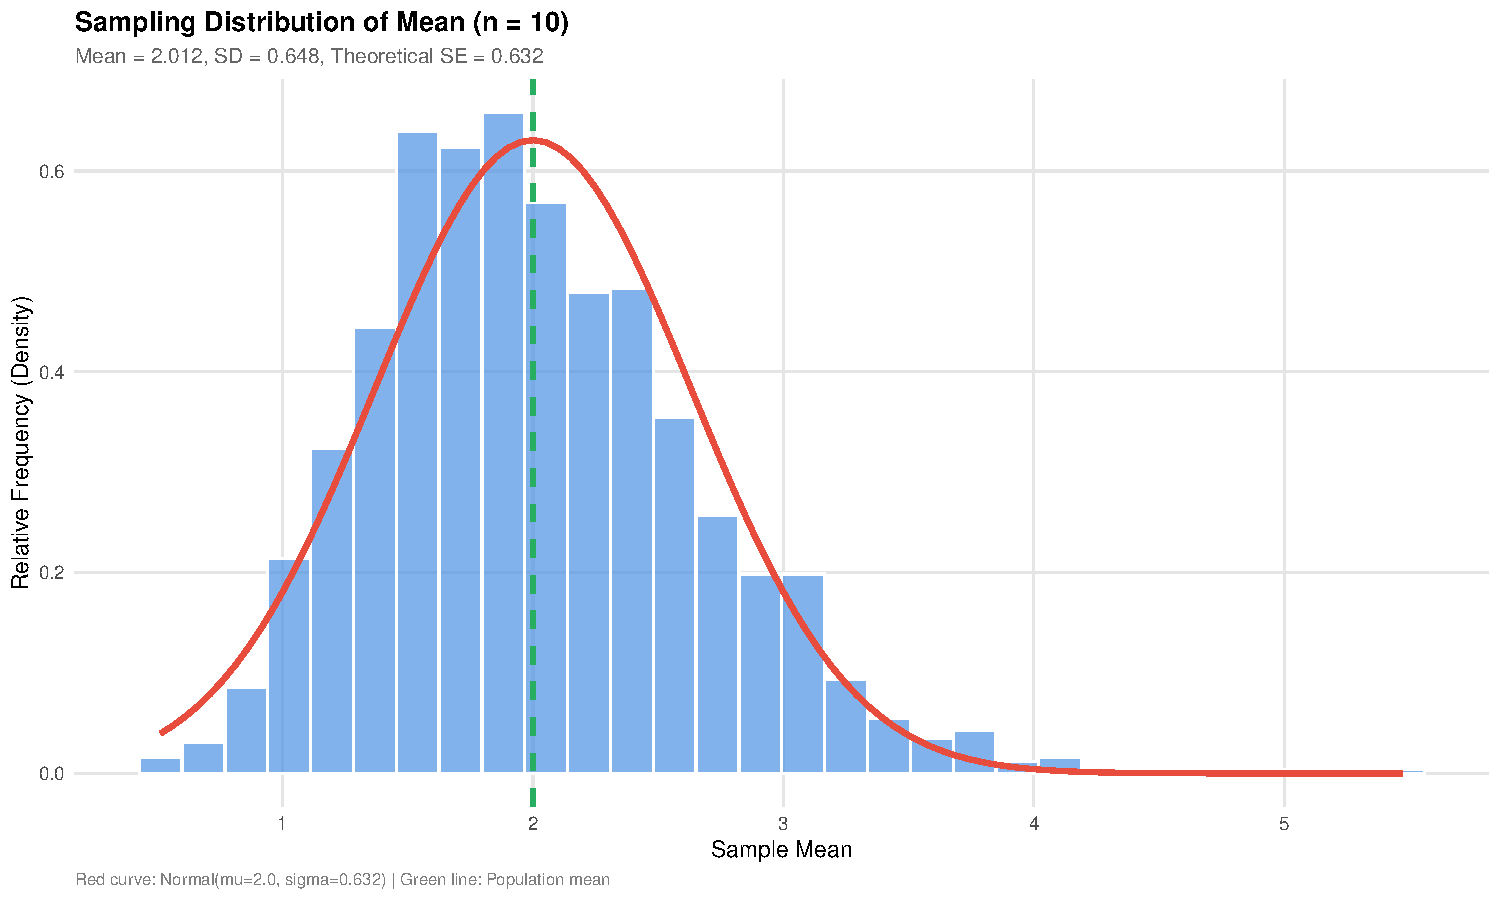
\includegraphics[width=0.7\textwidth]{../R/plots/sampling_distribution_n10.pdf}
    \caption{Sampling distribution for $n = 10$}
    \label{fig:n10}
\end{figure}

\begin{figure}[h]
    \centering
    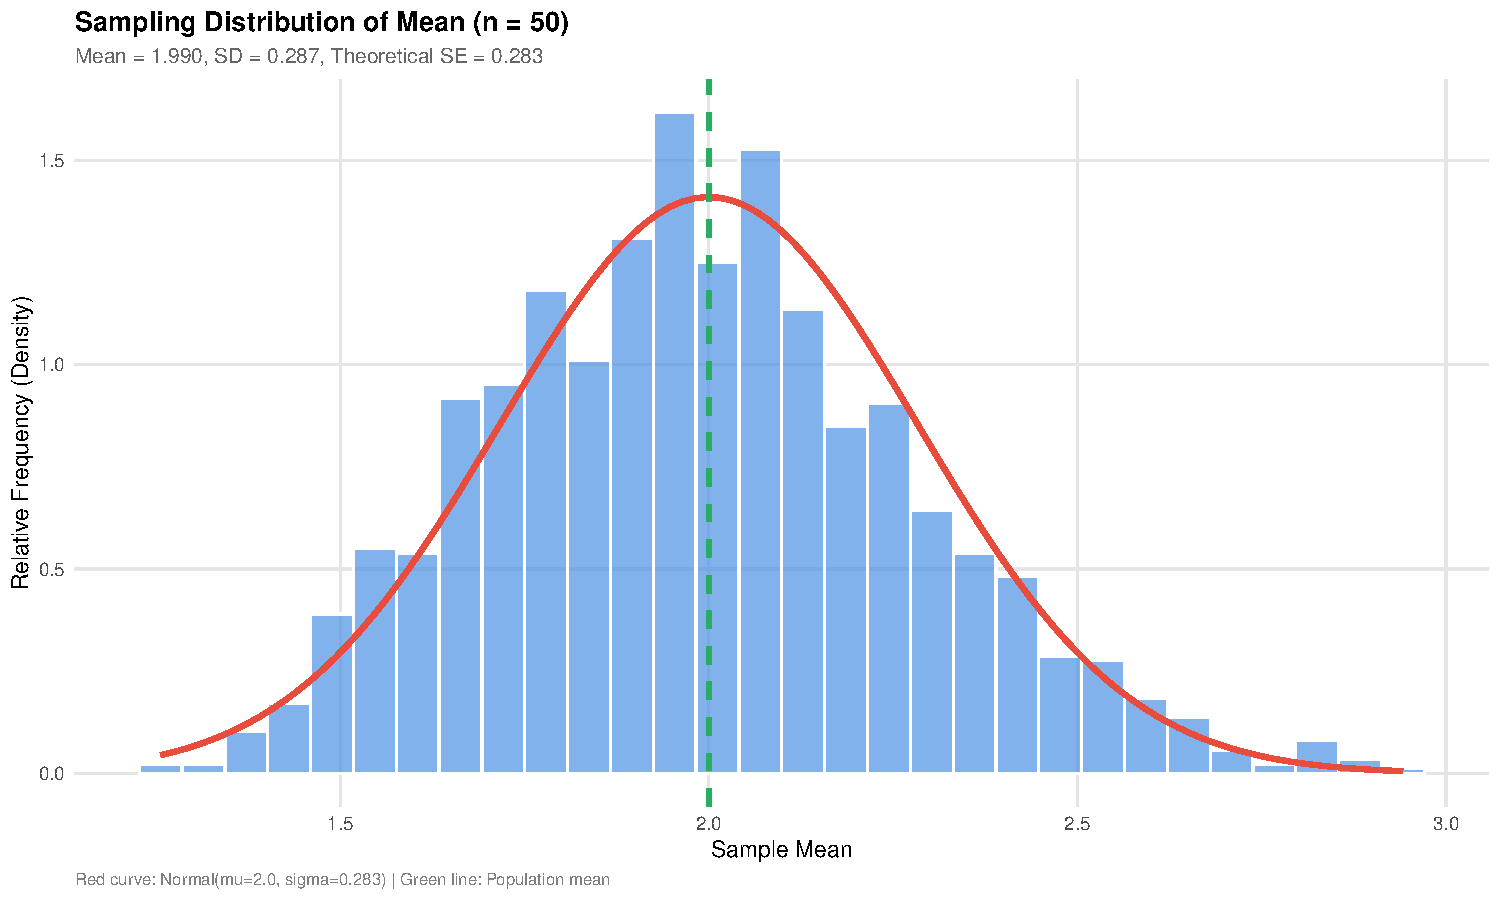
\includegraphics[width=0.7\textwidth]{../R/plots/sampling_distribution_n50.pdf}
    \caption{Sampling distribution for $n = 50$}
    \label{fig:n50}
\end{figure}

\begin{figure}[h]
    \centering
    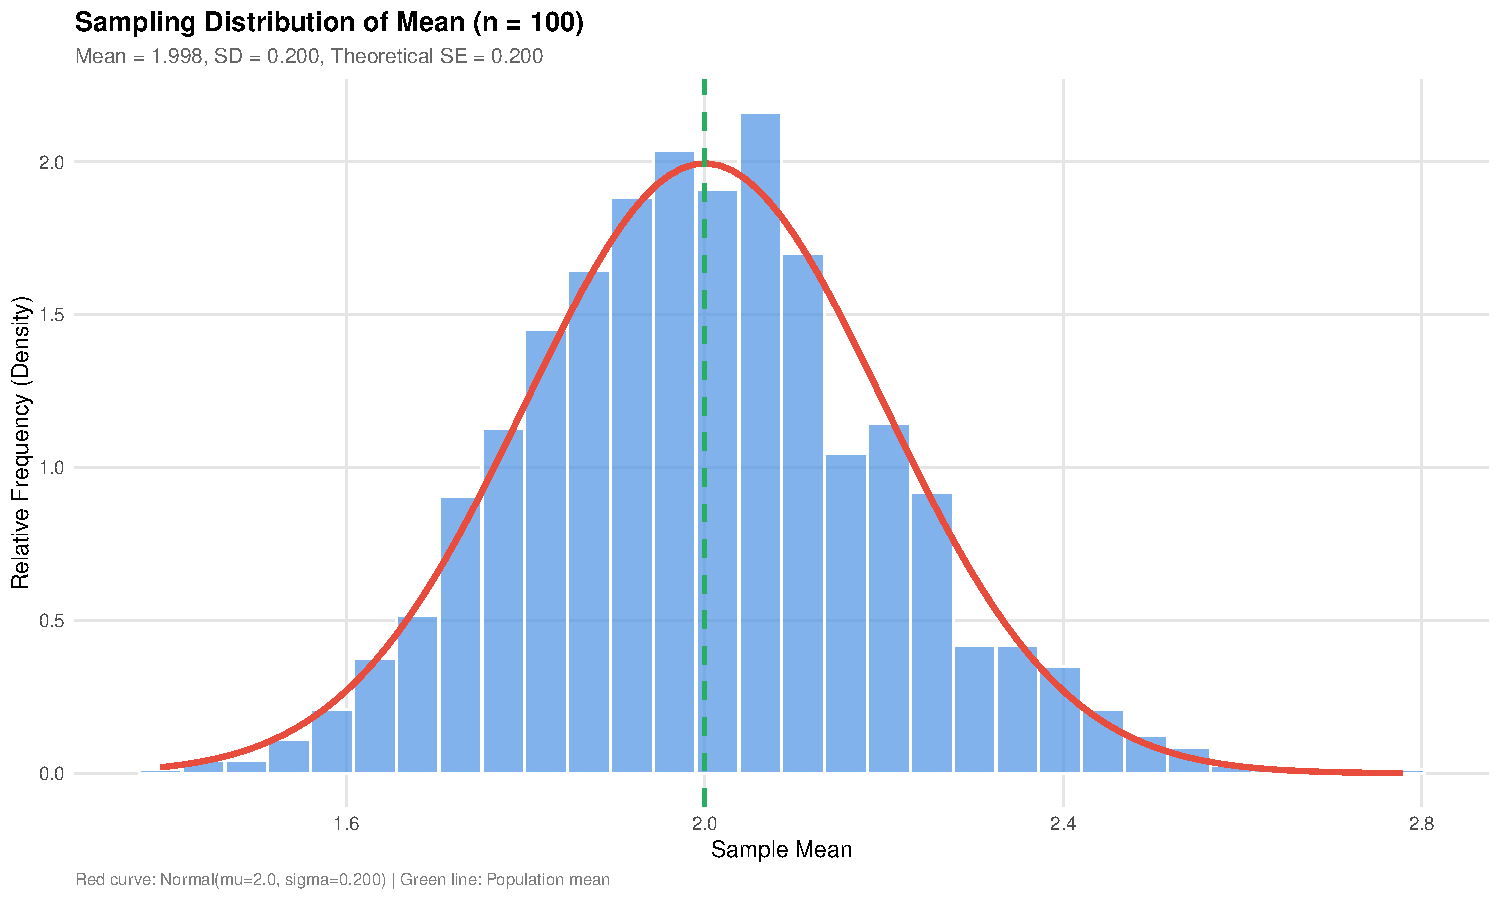
\includegraphics[width=0.7\textwidth]{../R/plots/sampling_distribution_n100.pdf}
    \caption{Sampling distribution for $n = 100$}
    \label{fig:n100}
\end{figure}

\begin{figure}[h]
    \centering
    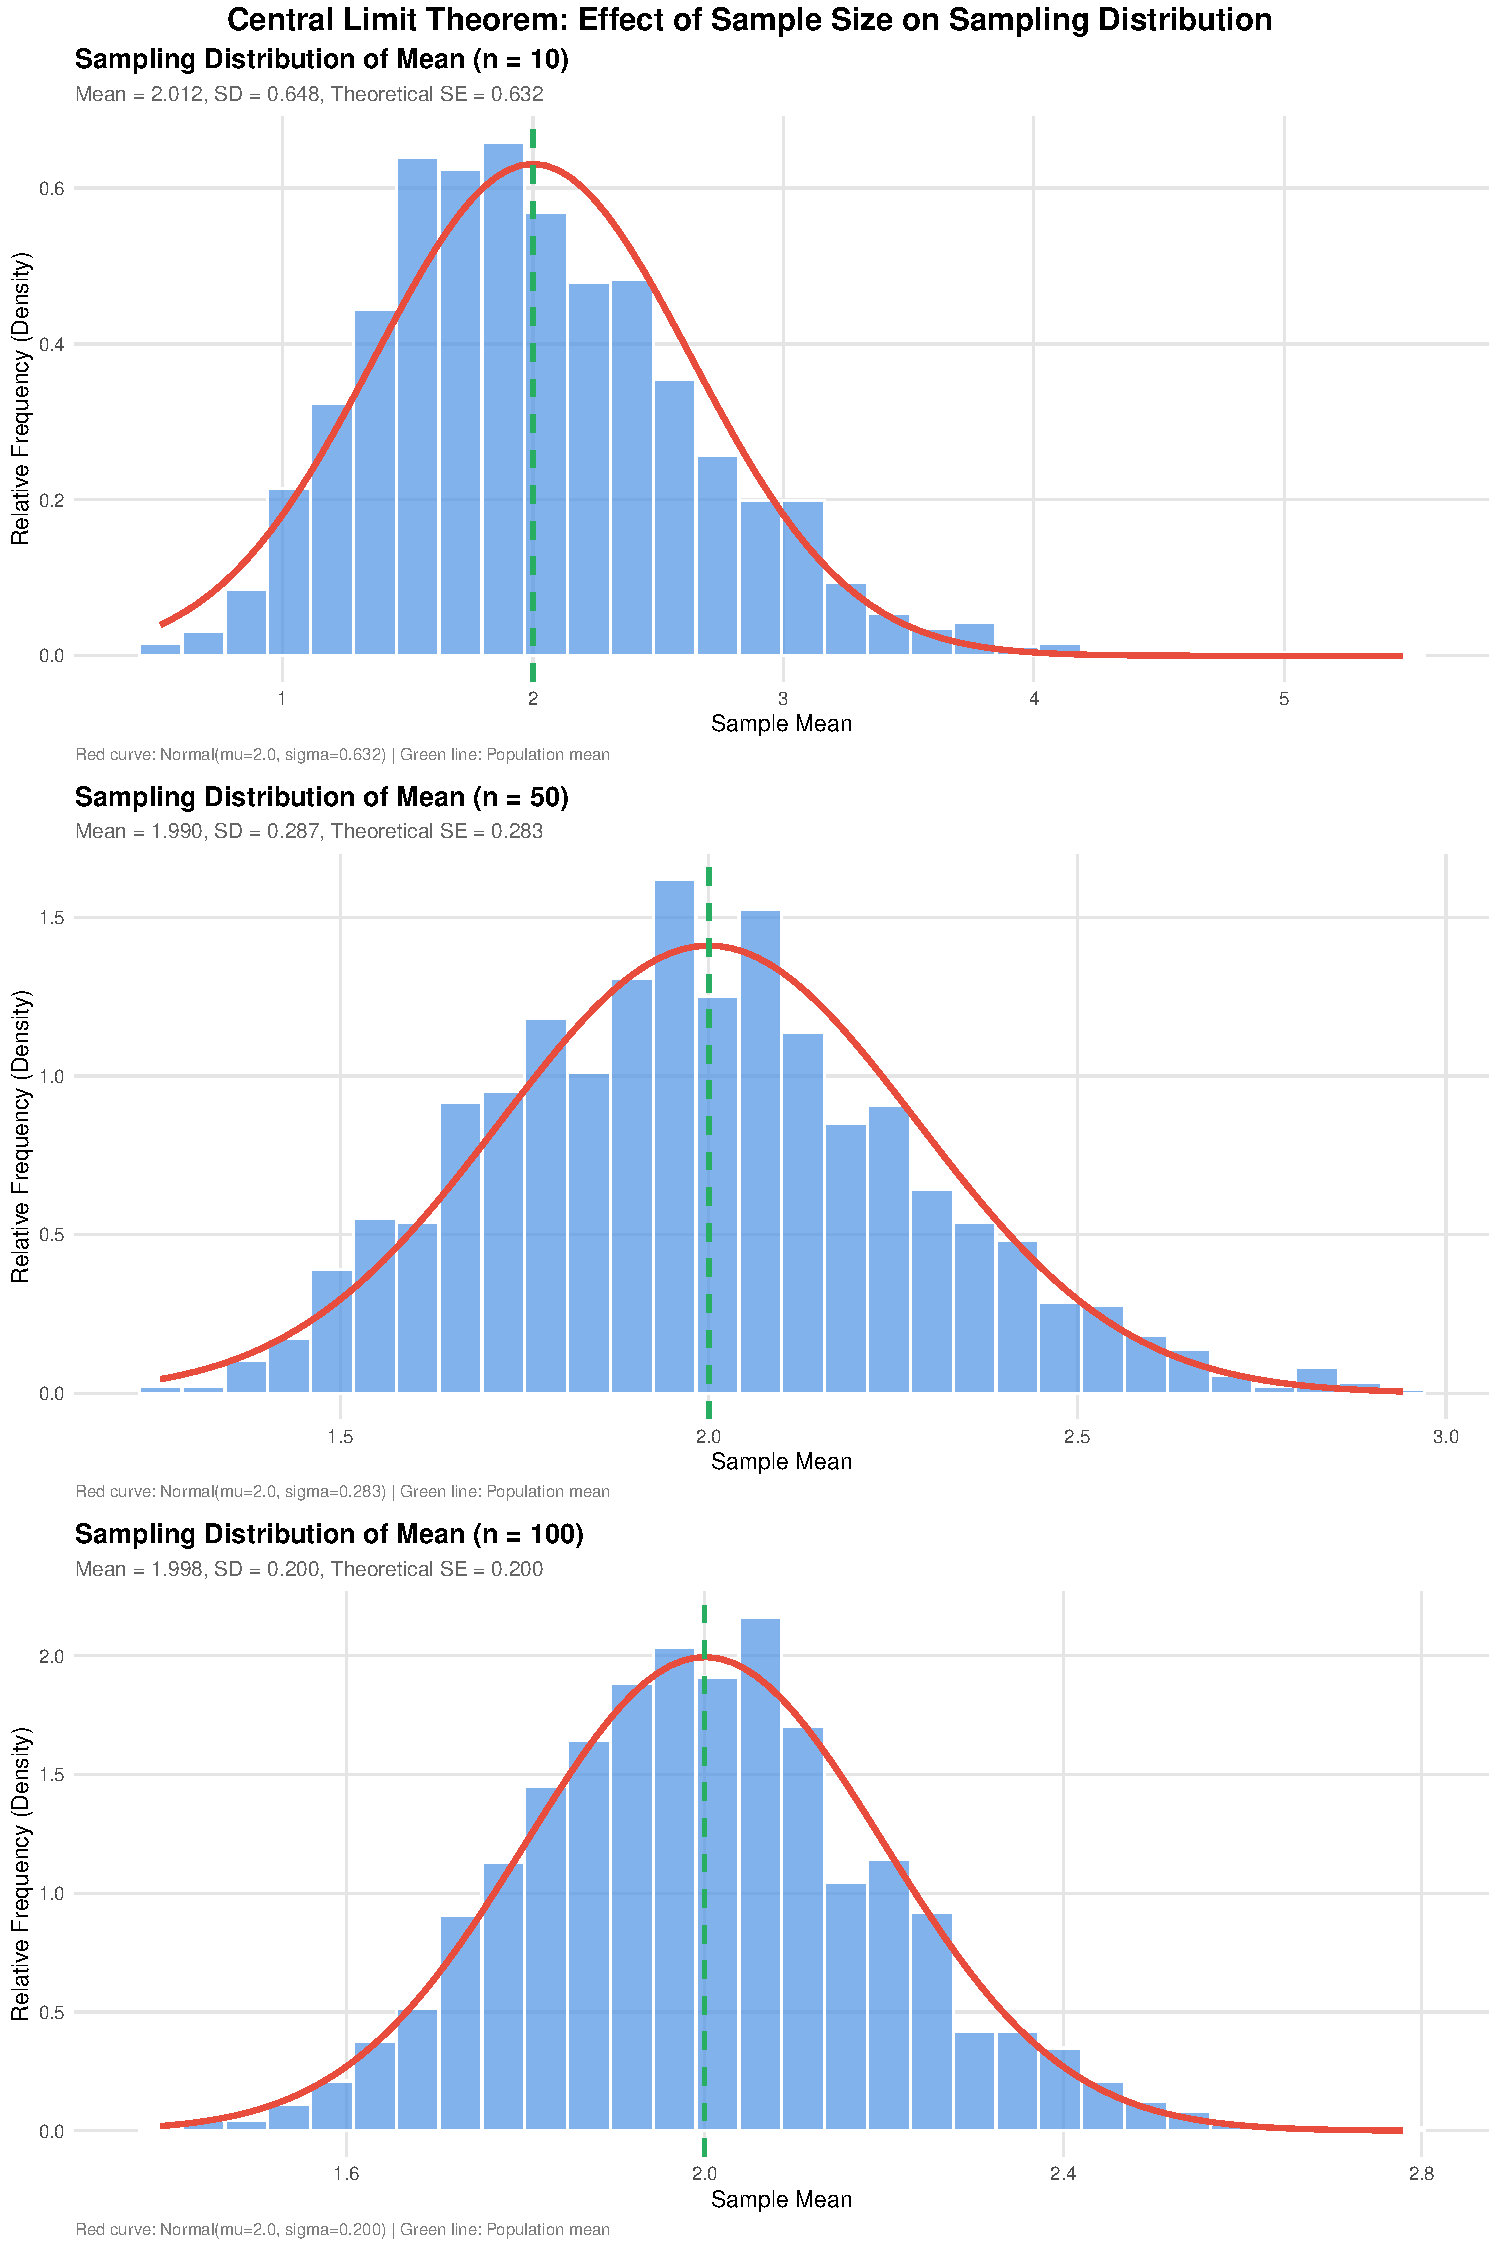
\includegraphics[width=0.9\textwidth]{../R/plots/sampling_distribution_combined.pdf}
    \caption{Combined sampling distributions for $n = 10, 50, 100$}
    \label{fig:combined}
\end{figure}

\end{document}